\documentclass[11pt]{artuppax}

\usepackage[utf8]{inputenc}

%\setdefaultlanguage[variant=british]{english}
\setdefaultlanguage{french}
\setmainlanguage{french}
\setotherlanguage[variant=us]{english}

%\title{Demande d'accueil en délégation au CNRS}
\title{Demande d'autorisation à diriger une thèse à l'UPPA}
\author{Germain Salvato Vallverdu}
\date{\today}
%\entete{Demande d'accueil en délégation au CNRS}
\entete{Curiculum Vitae Académique}
%\subentete{}
\HeaderUPPA

\usepackage[version=3]{mhchem}
%\setlength{\bibsep}{0pt plus 0.3ex}
%\geometry{a4paper, margin=2cm}
\usepackage{tabularx}

\usepackage[sectcntreset]{bibtopic}
\usepackage[numbers, sort&compress, super]{natbib}
\bibliographystyle{achemso_perso}

\usepackage[absolute,showboxes,overlay]{textpos}
\TPshowboxesfalse
\textblockorigin{2mm}{2mm}

\newcommand*{\bul}{~$\bullet$~\xspace}

\newcommand{\rubriq}[2]{
\vspace{2\parsep}
\begin{tikzpicture}
    \node[anchor=south west, font={\huge}, inner sep=0pt] at (0, 0) {\textsc{#1 :}};
    \node[anchor=south east, font=\LARGE] at (\textwidth, 0) {#2};
    \draw[ultra thick, black] (0, -.2) -- ++ (\textwidth, 0);
    %\node[fill=red] at (0, 0) {};
\end{tikzpicture}
\vspace{-8mm}}

\usepackage{url}
\usepackage{pdfpages}
\usepackage{fontawesome5} % need xelatex
\usepackage{graphicx}
\usepackage[hidelinks]{hyperref}

\usepackage{enumitem}
\setlist[itemize]{itemsep=2pt, topsep=0pt}
%\setlist{nosep}
%\setlength\itemsep{0pt}

\usepackage{titlesec}
\newcounter{subsec}[section]
\setcounter{subsec}{0}
\titleformat{\subsection}[hang]%
  {\bfseries\Large}%
  {\stepcounter{subsec}\thesubsec)}%
  {1ex}%
  {}%
  %[\vspace{-3ex}\rule{\textwidth}{0.75pt}]
\titlespacing*{\subsection}{0ex}{2ex}{0ex}

\titleformat{\subsubsection}[hang]{\bfseries}{}{0ex}{}
\titlespacing*{\subsubsection}{0ex}{0ex}{-1ex}


\fancypagestyle{titlepage}{%
        \fancyhead{}%
        %\fancyhead[C]{\includegraphics[height=2cm]{\@uppalogo}}
        \fancyfoot[R]{{}}%
        \fancyfoot[L]{}%
        \fancyfoot[C]{%
            {\color{black} UNIVERSIT\'E DE PAU ET DES PAYS DE L'ADOUR}%
            \begin{tikzpicture}[overlay, remember picture]
                \draw[thick, black] ($(current page.south west) + (0,1cm)$) --
                    ($(current page.south east) + (0,2cm)$);
            \end{tikzpicture}%
        }
    }

\renewcommand{\maketitle}{%
    \thispagestyle{titlepage}
    \singlespacing
    \begin{center}
        \parbox{.33\textwidth}{\includegraphics[height=2cm]{logotype_iprem}}
        \parbox{.33\textwidth}{\centering 
\includegraphics[height=2.5cm]{LogoUPPAcouleurRVB}}
        \parbox{.33\textwidth}{\hfill\includegraphics[height=2.2cm]{CNRS}}

        \vspace*{\stretch{1}}

        {\Huge\bfseries\setlength{\baselineskip}{1.2\baselineskip}%
        %Dossier de demande d'accueil en délégation au CNRS
        %Dossier de demande d'un congé pour recherches ou conversions thématiques
        Demande d'autorisation à diriger une thèse à l'UPPA
        \par}

        \vspace{4ex}

        {\LARGE Germain SALVATO VALLVERDU}

        {\Large IPREM - UMR 5254}

        {\Large\itshape\today}

    \end{center}
    \vspace*{\stretch{1}}
    }

% ------------------------------------------------------------------------------

\begin{document}

%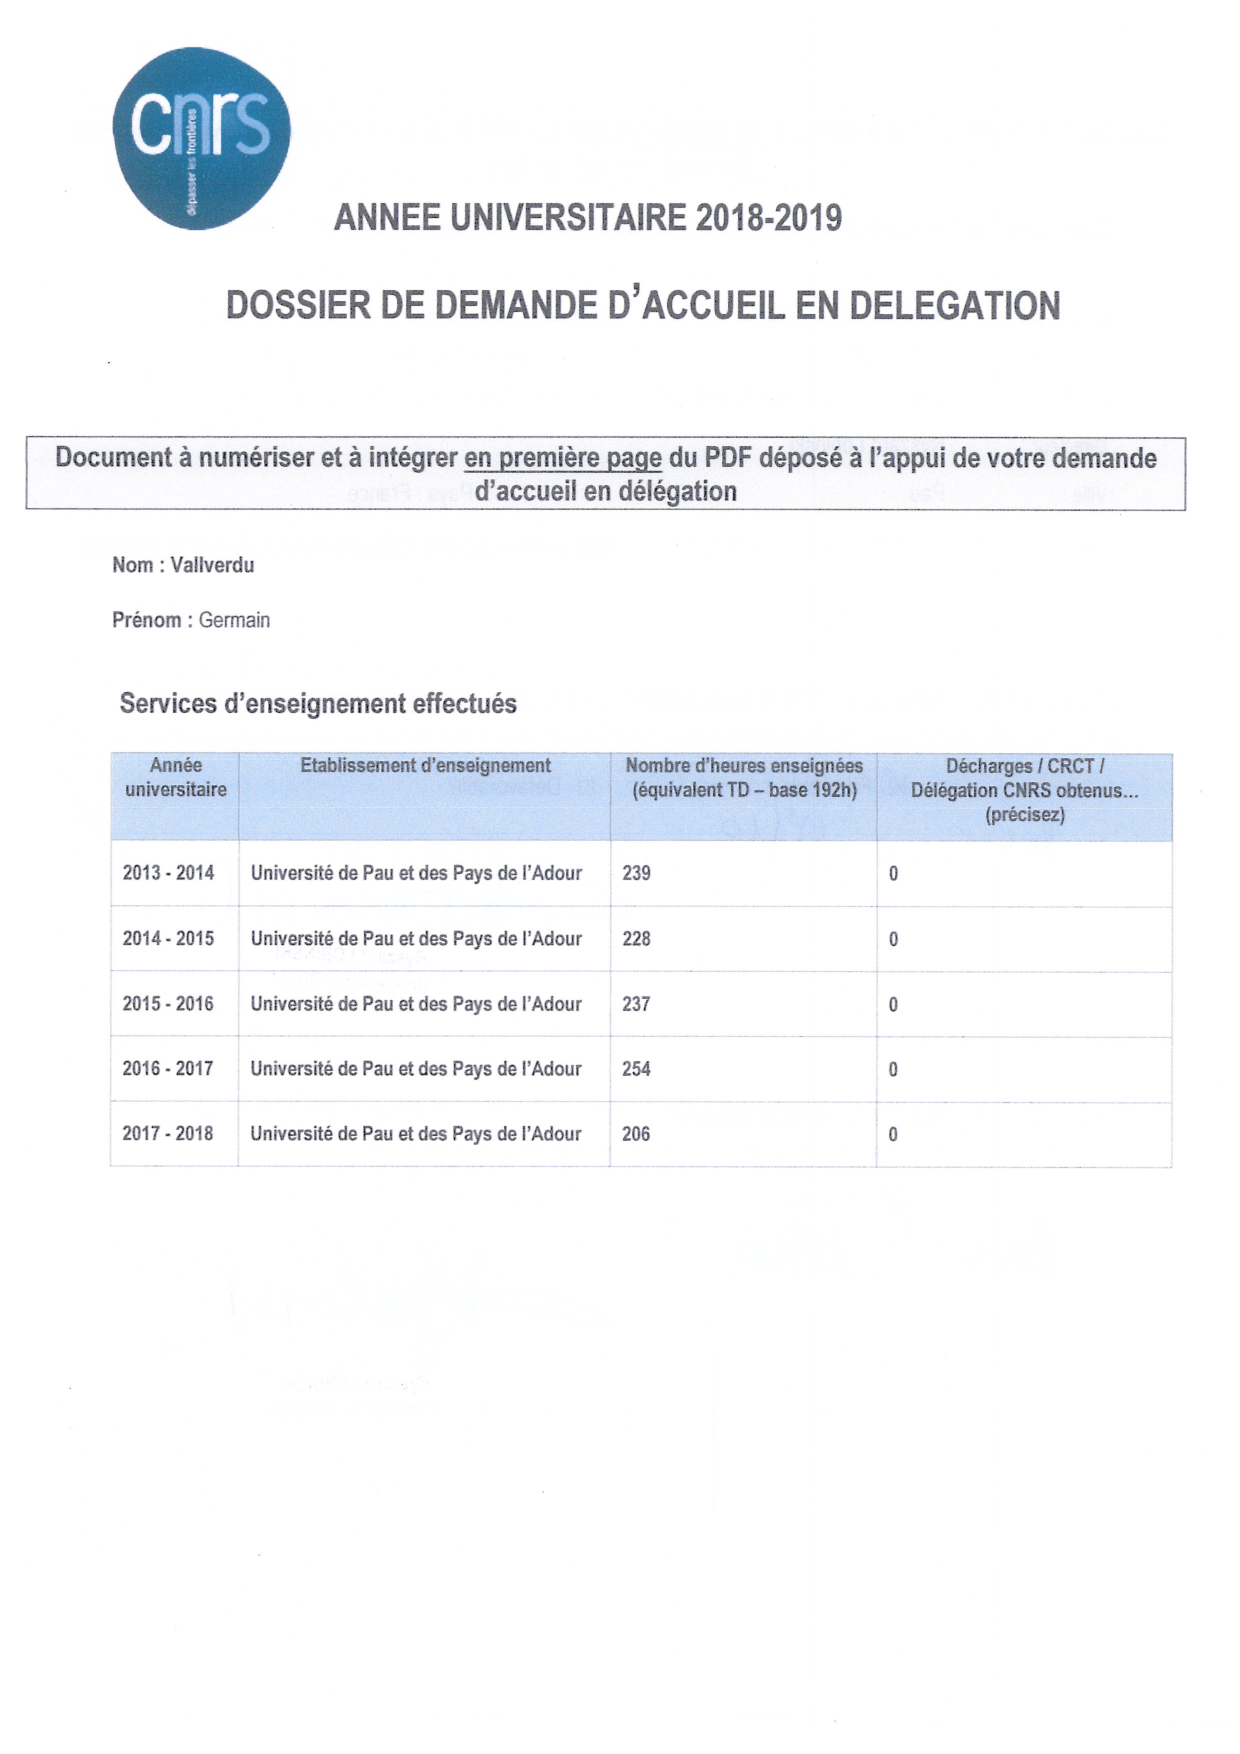
\includepdf[pages=1,scale=1]{formulaire.pdf}
%\includepdf[pages=2,scale=1, angle=180]{formulaire.pdf}

\maketitle

\newpage
\setcounter{tocdepth}{1}
\tableofcontents

\newpage

\addcontentsline{toc}{section}{1. Demande de direction de thèse}
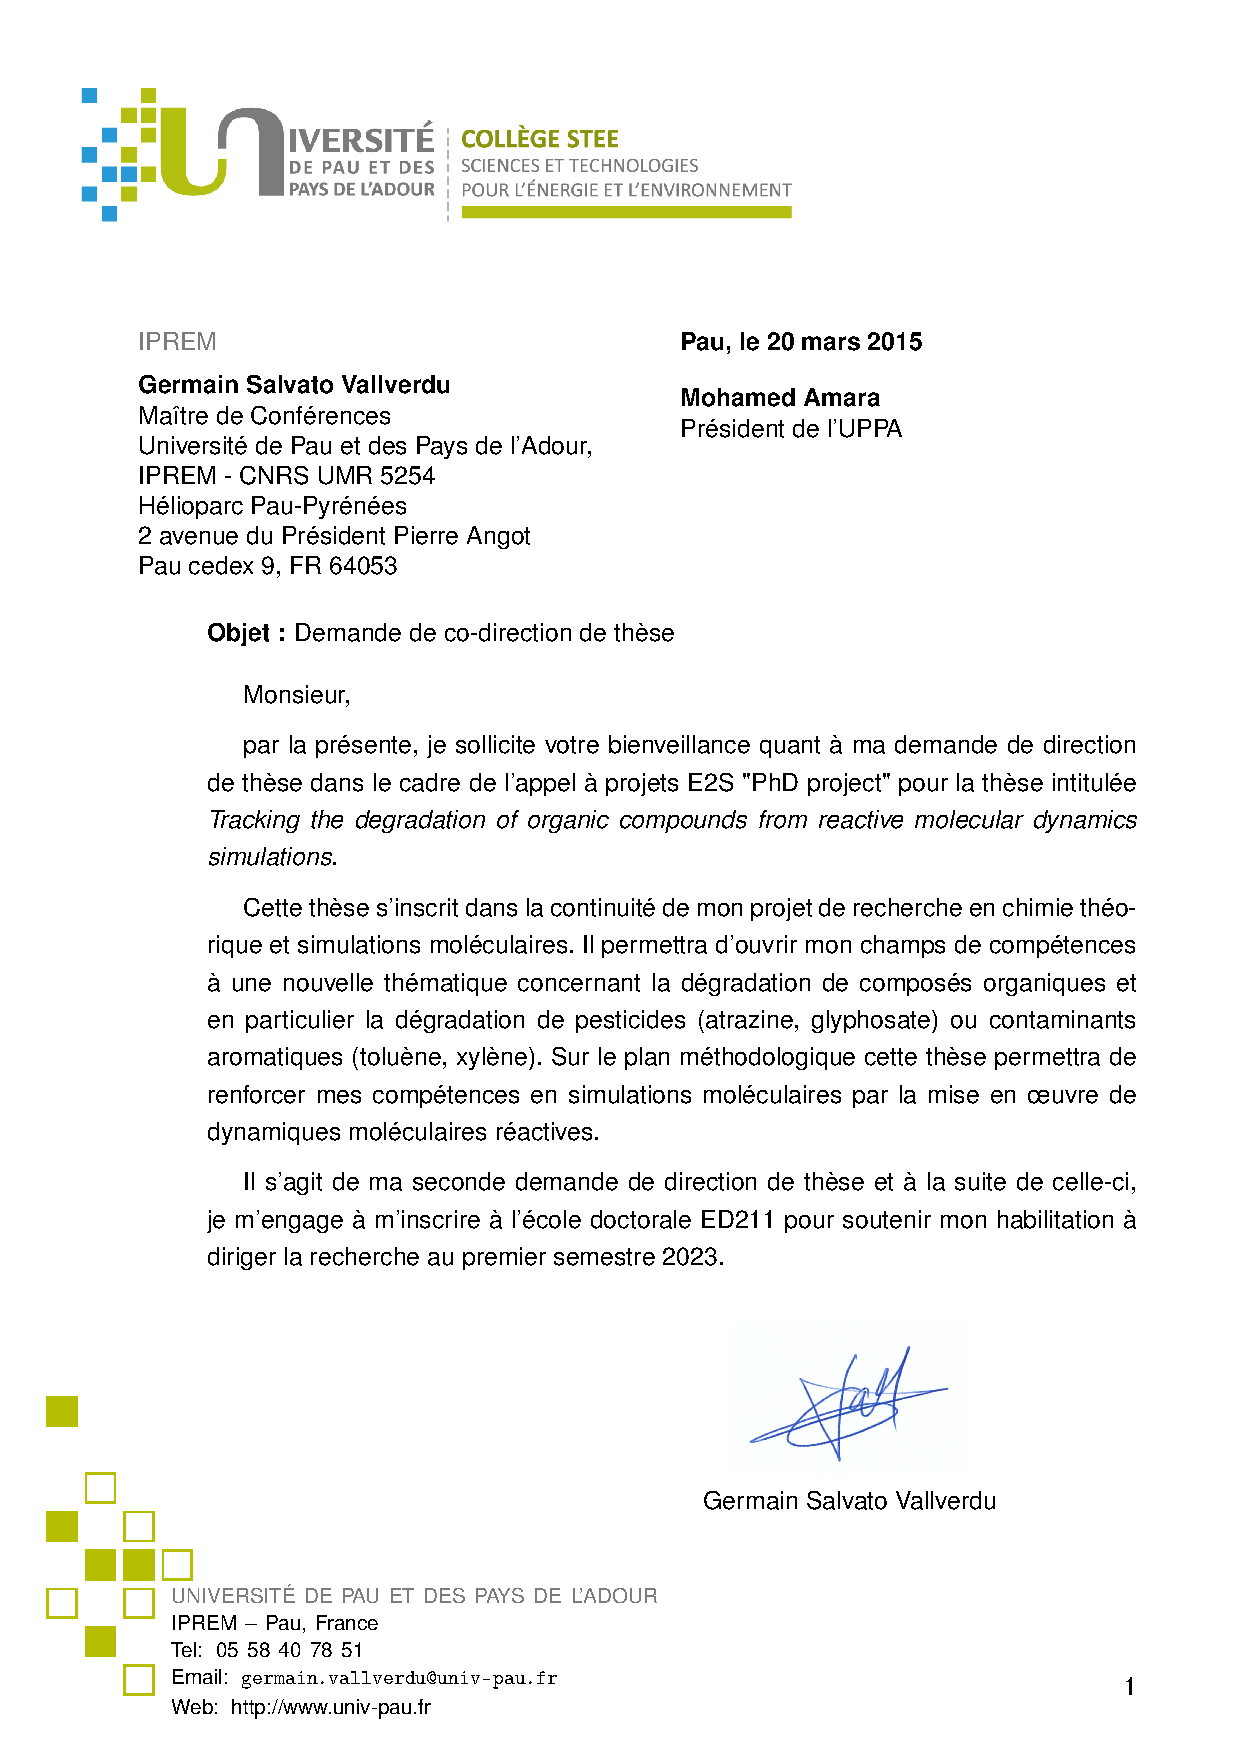
\includepdf[scale=1]{lettre.pdf}
\stepcounter{section}

\includepdf[scale=1]{ficheED.pdf}


\addcontentsline{toc}{section}{2. Curiculum Vitae court}
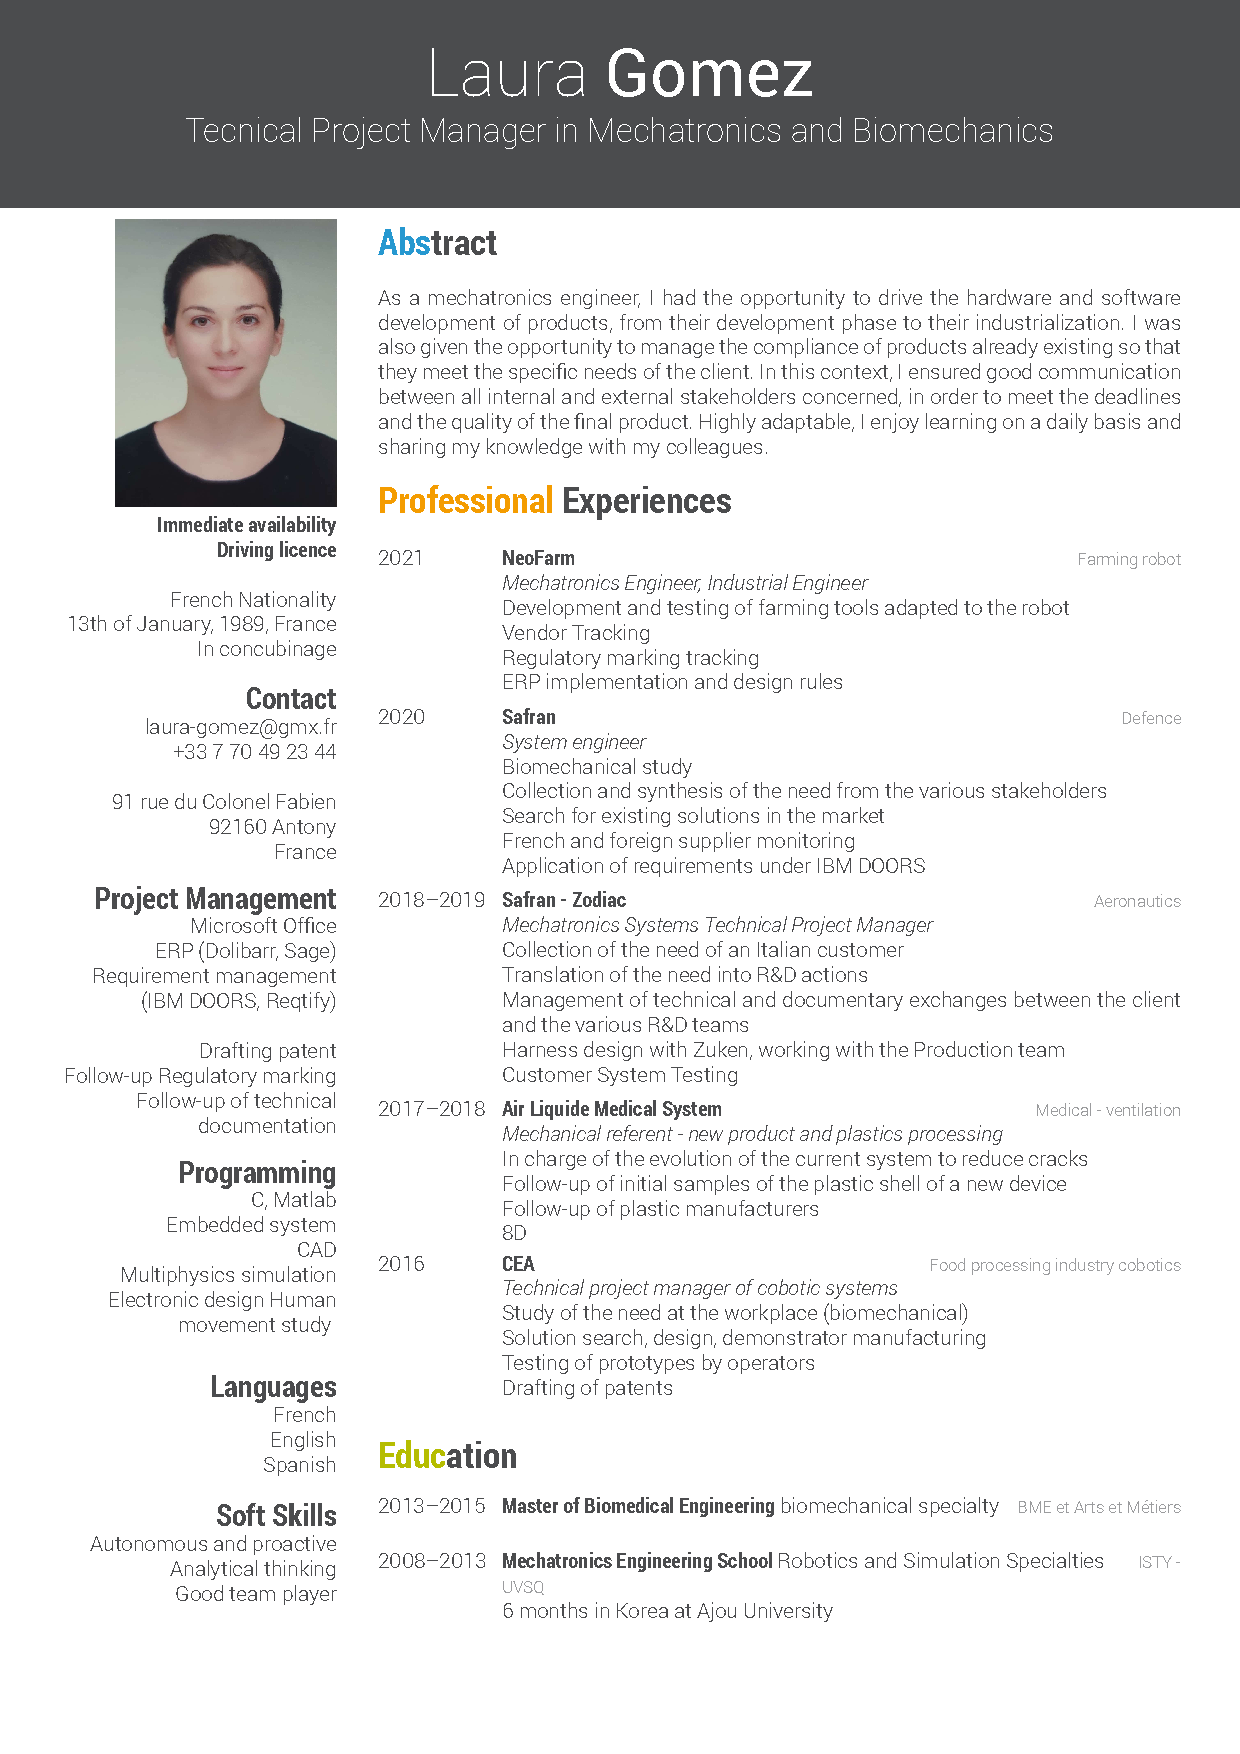
\includepdf[scale=1]{../cv-en-short.pdf}
\stepcounter{section}

%\section{Curiculum Vitae}

%\vspace*{5mm}
\begin{center}
    \LARGE
    \textsc{Curiculum Vitae}
\end{center}
\vspace*{10mm}
\addcontentsline{toc}{section}{3. Curiculum Vitae}

	\begin{textblock*}{60mm}(12cm,6cm)
	    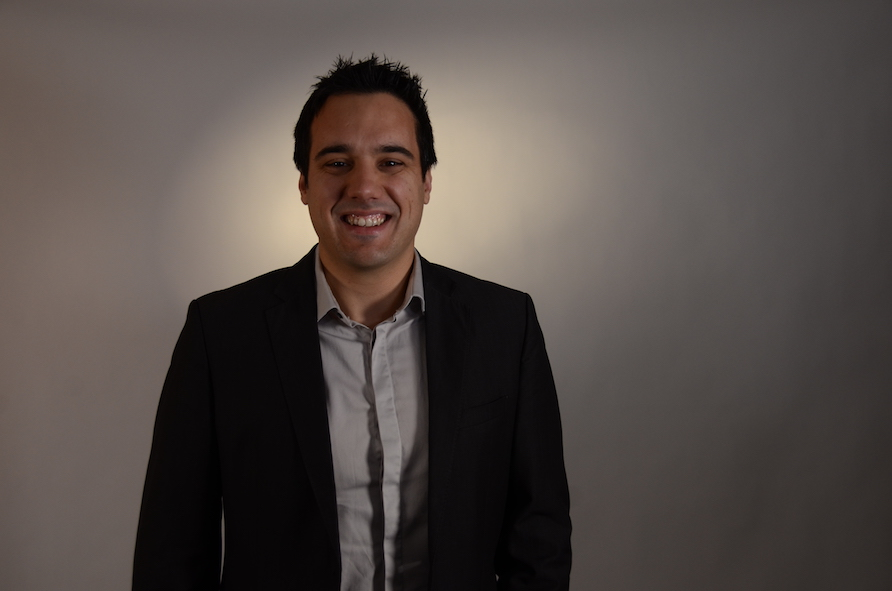
\includegraphics[height=4cm]{gvallver}
	\end{textblock*}


\textbf{\large Germain \textsc{Salvato Vallverdu}} \\
Nationalité française \\
Né le 10 Août 1983 à Perpignan (Pyrénées orientales) \\
Marié, 2 enfants


\faFlask{} IPREM\\
Technopôle Hélioparc\\
2 avenue du Président Pierre Angot\\
64053 Pau Cedex 9\\
\faPhone{} 05 59 40 78 51\\
\faAt{} germain.vallverdu@univ-pau.fr \par

\faNewspaper{} \url{https://publons.com/researcher/2764008/} \\
%$\vcenter{\hbox{
\includegraphics[height=5mm]{../img/iD-icon}}}$ \url{orcid.org/0000-0003-1116-8776}\\
\faGithub{} \url{@gvallverdu} \quad - \quad \url{https://github.com/gVallverdu/}\\
\faGlobe{} \url{http://gvallver.perso.univ-pau.fr}

\singlespacing
\rubriq{Fonctions}{\faBlackTie}

\begin{description}
	\item \textbf{Octobre 2010 \faArrowCircleRight{} Aujourd'hui} \hfill \textit{Maître de conférences}
	\begin{itemize}
		\item Chimie théorique, modélisation moléculaire, simulation numérique.
		\item Université de Pau et des Pays de l'Adour
		\begin{itemize}
		    \item Matrices complexes, pétrochimie, thermochimie
		    \item Bio-dégradation de composés organiques
		    \item Processus électroniques dans les matériaux pour le stockage électrochimique de l'énergie
		\end{itemize}
	\end{itemize}

	\item \textbf{2009 \faArrowCircleRight{} 2010} \hfill \textit{Chercheur-Ingénieur}
	\begin{itemize}
	    \item Développement et implémentation d'un modèle mésoscopique pour
	    l'étude de la propagation d'ondes de chock réactives.
		\item CEA - DAM Île de France.
	\end{itemize}

	\item \textbf{2006 \faArrowCircleRight{} 2009} \hfill \textit{Allocataire Moniteur}
	\begin{itemize}
	    \item Étude théorique de processus photophysiques dans des
		protéines fluorescentes.
		\item Université Paris Sud 11, Laboratoire de Chimie Physique, Orsay
	\end{itemize}
\end{description}

\newpage
\rubriq{Formation}{\faGraduationCap}

\begin{description}
	\item \textbf{16 Juillet 2009 \bul Soutenance de thèse}
	\begin{description}
		\item \textbf{Titre : } Étude théorique de processus photophysiques dans des
		protéines fluorescentes.
		\item financement MNRT, mention très honorable.
		\item \textbf{Composition du jury : }
		\begin{itemize}
			\item M. David Perahia (Directeur de recherche, IBBMC, Université Paris-Sud 11),
				\textit{président}
			\item M. Xavier Assfeld (Professeur, Université Henry Poincaré, Nancy),
			\textit{rapporteur}
			\item M. Daniel Borgis (Directeur de recherche, ENS Paris), \textit{rapporteur}
			\item M. Olivier Parisel (Directeur de recherche, lCT, Université Paris 6)
			\item Mme Fabienne Mérola (Directeur de recherche, LCP, Université Paris-Sud 11)
			\item Mme Isabelle Demachy (Professeur, LCP, Université Paris-Sud 11),
				\textit{directrice de thèse}
		\end{itemize}

		\item \textbf{Disponible sur Thèse en ligne}
			\begin{itemize}
				\item \url{http://tel.archives-ouvertes.fr/tel-00431879/fr/}
			\end{itemize}
	\end{description}

	\item \textbf{2006 - 2009 \bul Doctorat : Allocataire Moniteur à l'université Paris-Sud 11}
	\begin{itemize}
		\item[] Travaux de recherche effectués dans le Laboratoire de Chimie Physique,
		UMR 8000, financement MNRT, mention très honorable.
		\item[] Enseignements effectués à l'IUT de mesures physiques d'orsay.
	\end{itemize}

	\item \textbf{2003 - 2006 \bul Magistère de Physico-Chimie Moléculaire}
	\begin{description}
		\item Université Paris-Sud 11 et Ecole Normale Supérieure de Cachan.
	\end{description}

	\item \textbf{2004 - 2006 \bul Master de Physico-Chimie Molécualire}
	\begin{description}
		\item Université Paris-Sud 11, mention Très Bien.
	\end{description}

	\item \textbf{2003 - 2004 \bul Licence de Chimie Physique}
	\begin{description}
		\item Université Paris-Sud 11, mention Très Bien.
	\end{description}

	\item \textbf{2001 - 2003 \bul Classes préparatoires aux grandes écoles}
	\begin{description}
		\item Lycée François Arago (Perpignan), classes PCSI - PC.
	\end{description}

\end{description}

\onehalfspacing

% ------------------------------------------------------------------------------

\newpage

\rubriq{Activités de recherche}{\faCog}
\addcontentsline{toc}{section}{4. Activités de Recherche}
\stepcounter{section}

\subsection{Résumé}

Mes activités de recherche concernent le développement de nouvelles méthodes de chimie théorique et de nouvelles stratégies calculatoires pour l'étude de systèmes complexes à différentes échelles de temps ou d'espace. Dans ce cadre je dispose d'une forte expérience dans les méthodes de chimie théorique et simulations allant des méthodes de chimie quantique à la dynamique moléculaire de systèmes moléculaires ou mésoscopiques. L'association de ces méthodes de simulation permet d'aborder la problématique d'intérêt en considérant toutes les facettes du système et d'être au plus prêt des conditions expérimentales. Il s'agit, d'une part, de concevoir un modèle pertinent qui est capable d'avoir un comportement similaire à un système réel ou d'en reproduire la partie d'intérêt ; et, d'autre part, de choisir les méthodes de simulations adaptées qui seront techniquement envisageables et donneront des résultats avec une précision suffisante pour répondre aux questions posées. La précision des résultats obtenus par les approches théoriques et assujetti à la précision de la description des interactions entre les constituants du système étudié : interactions inter-atomiques pour la structure moléculaire, interactions inter-moléculaires pour la phase condensée ou les systèmes biologiques, interaction molécule/surface ou molécule/agrégat pour la réactivité chimique. En conséquence, le développement et la mise en œuvre de méthodes permettant de décrire ces interactions de la façon la plus précise et pertinente possible est au centre de mes activités de recherche.

Un autre dénominateur commun de mes sujets de recherche est l'interaction et le dialogue avec une partie expérimentale. Cette approche couplée entre techniques expérimentales et méthodes théoriques permet à chaque discipline de s'enrichir mutuellement et d'agir en synergie pour répondre aux questions posées. Dans ce contexte, je me suis intéressé à plusieurs domaines d'applications en lien soit avec le stockage électrochimique de l'énergie, soit avec l'étude de matrices complexes dans le domaine pétrolier.

L'IPREM est l'un des membres fondateurs du Réseau Français pour le Stockage Électrochimique de l'énergie (RS2E)\footnote{\url{http://www.energie-rs2e.com/}}. Dans ce contexte, en collaboration avec les techniques de caractérisation de surface disponibles à l'IPREM, nous étudions les propriétés de surface des matériaux d'électrodes ainsi que les processus ayant lieu aux interfaces électrode-électrolyte. La proportion de surfaces et interfaces dans les matériaux de batteries étant importante, ces processus ont un fort impact sur les performances électrochimiques de ces systèmes. Dans cette thématique j'ai participé à l'encadrement de plusieurs thèses. La thèse de Lucile Martin (2010-2013) concernait l'étude des interfaces solides-solides dans les microbatteries à base de cuivre et a permis de mettre en évidence la structure et la composition chimique des interfaces thermodynamiquement les plus stables. J'ai ensuite co-dirigé la thèse d'Èmilie Guille (2011-2014) concernant les interfaces entre une électrode et le LiPON, un électrolyte solide. Nous avons d'une part proposé un modèle structural pour le LiPON qui est un verre et étudié les processus de diffusion du lithium à l'interface. J'ai ensuite participé à l'encadrement de thèse d'Ambroise Quesne-Turin (2014-2017) et je participe à celui d'Alexia Lemoine (2018-2021) concernant l'étude de la réactivité de surface de matériaux d'électrodes par une approche couplée expérience théorie.

Depuis 2016, dans le cadre du laboratoire commun \textit{Complex Matrices Molecular Characterization} (C2MC) nous étudions les propriétés physico-chimiques de matrices complexes issues du pétrole lourd. Il s'agit, d'une part, de comprendre les processus d'agrégation, de précipitation et de solubilité d'une classe de molécules présente dans le pétrole, les asphaltènes ; et, d'autre part, de préciser la connaissance des structures chimiques de cette famille de molécule. Ces travaux, se font en collaboration avec le groupe Total et donnent lieu a des activités de développement pour la mise au point des champs de forces des systèmes étudiés et à la production de simulations de dynamiques moléculaires classiques. Je participe à l'encadrement de deux étudiants actuellement en thèse dans cette thématique, Bhuvan Kumar Gunessee (2018-2021) et Orlando Villegas (2017-2020) en cotutelle avec l'Universidad Central de Venezuela.

\subsection{Encadrements}

\subsubsection{Encadrement doctoral}

Depuis mon recrutement j'ai participé à l'encadrement des thèses de
Lucile Martin (2010-2013), Ambroise Quesne-Turin (2014-2017),
Alexia Lemoine (2018 - 2021), Bhuvan Kumar Gunessee (2018 - 2021)
et Orlando Villegas (2018 - 2021).

\textbf{Émilie Guille (2011-2014)} :
L'école doctorale ED211 et l'UPPA m'ont accordé une co-direction
à hauteur de 40\% avec le Pr Isabelle Baraille pour cette thèse.

Cette thèse a concerné l'étude de l'interface entre une électrode et un électrolyte
solide. Ce type d'électrolyte est utilisé pour contourner les problèmes de sécurité
inhérents aux électrolytes liquides dans des microbatteries au lithium. L'électrolyte
étudié était le \ce{Li_xPO_yN_z} (LIPON) qui présente une structure amorphe. La plus
longue partie de la thèse fut consacrée à l'identification de motifs représentatifs de
la structure du LIPON par comparaison de résultats expérimentaux et théoriques :
spectres IR, Raman, XPS. Le modèle a ensuite été utilisé pour étudier l'interface
entre le LIPON et une électrode modèle de silicium.

\subsubsection{Encadrements d'étudiants en M2 Recherche}

Depuis 2013 j'ai encadré 8 étudiants en Master 2 chimie et physico-chimie des matériaux,
spécialité recherche. 4 d'entre eux ont travaillé sur des sujets mixtes couplant expériences
et théorie en collaboration avec un expérimentateur de l'IPREM spécialiste de la caractérisation de
surface. Les noms, dates, taux d'encadrement et les titres des stages sont reportés
dans le tableau ci-dessous.


{\singlespacing
\renewcommand{\arraystretch}{1.2}
\begin{tabularx}{\textwidth}{lllX}
\hline
Nom de l'étudiant & année & taux & sujet \\
\hline
Marie Minvielle & 2013 & 50\% & Étude de l'adsorption de sondes gazeuses à la surface de
                                matériaux d'électrode positive: couplage expérience/théorie \\
Dimitri Del Pianta & 2014 & 50\% & Étude des processus d'insertion dans les matériaux
                                   d'électrode positive pour microbatteries au sodium \\
William Lafargue-Dit-Hauret & 2015 & 100\% & Étude théorique de la conductivité ionique à
                                     l'interface
                                     électrode/électrolyte solide: Application au système
                                     LiPON/Si\\
Youn Charles-Blin & 2016 & 50\% & Étude de la réactivité de surface de matériaux d'électrode
                                  modèles de la famille des oxydes de lithium lamellaire:
                                  approche couplée expérience/théorie\\
Amine Bekkali & 2017 & 50\% & Une étude via un couplage expérience-théorie des déplacements
                              chimiques en spectroscopie photoélectronique à rayonnement X\\
Guillaume Fradet & 2017 & 50\% & Calculs de spectres Infra Rouge.\\
Gérald Munoz & 2018 & 50\% & La réactivité des porphyrines : applications aux fluides pétroliers\\
Quentin Labarde & 2019 & 50\% & Prévision de la viscosité d'un diesel paraffinique modèle par modélisation moléculaire\\
\hline
\end{tabularx}
}

%\subsection{Participation à un comité de sélection}
%
%En 2013, j'ai participé au comité de sélection pour le recrutement d'un Maître de
%conférence en section CNU 33 et 31. Le profil du poste concernait la
%Physico-chimie des matériaux appliquée aux surfaces / interfaces.

\subsection{Projets}

\begin{itemize}
    \item Demande d'Allocations de Ressources Informatiques (DARI)
    {\singlespacing
    \begin{itemize}
        \item 2018 - 2 500 000 heures scalaires
        \item 2017 - 1 000 000 heures scalaires
        \item 2016 - 400 000 heures scalaires
        \item 2015 - 200 000 heures scalaires
        \item 2014 - 200 000 heures scalaires
        \item 2013 - 150 000 heures scalaires
    \end{itemize}}
    \item 2016 - participation à la rédaction du Projet ANR INGROwTH (Rejeté à la deuxième étape).
    \item 2018/2019 - soumission de l'ANR JCJC MALICE
    \item 2018 - Projet région Nouvelle Aquitaine (IPREM - ICMCB (Bordeaux) - Saft (Partenaire industriel)), démarrage septembre 2018.
\end{itemize}



\newpage
\rubriq{Activités d'enseignement}{\faEdit}
\addcontentsline{toc}{section}{5. Activités d'enseignement}
\stepcounter{section}

J'effectue l'essentiel de mon service d'enseignement en chimie-physique :
\begin{itemize}\singlespacing
    \item Atomistique, L1 Physique-Chimie, Cours (9.5 HETD) /TD (10.5 HETD)
    \item États de la matière, L1 Physique-Chimie, TD (10.5 HETD)
    \item Atomistique et liaisons chimiques, L2 Chimie et Physique-Chimie, TD (19.5 HETD)
    \item Outils pour la symétrie moléculaire, L2 Chimie, Cours (9.5 HETD) / TD (10.5 HETD)
    \item Outils informatiques pour les sciences de l'ingénieur, L1, Cours/TD/TP (27 HETD)
%
%    \item Travaux pratiques de techniques de séparation et d'analyse, L2 Chimie et Biologie (20 HETD)
    \item Travaux pratiques de catalyse chimique, L2 Chimie (20 HETD)
    \item Travaux pratiques de thermochimie et cinétique chimique, L2 Chimie (20 HETD)
    \item Travaux pratiques de structure et réactivité des molécules, L3 Chimie (16 HETD)

    \item Structure électroniques des solides, M1 Chimie et Physico-Chimie des Matériaux, TD (10.5 HETD).
   \item Modélisation des matériaux à propriétés spécifiques. M1 Chimie et Physico-Chimie des Matériaux, Cours/TD (10 HETD).
\end{itemize}

En parallèle des enseignements de chimie-physique, je met en œuvre d'autres enseignements plus originaux par leur format (pédagogie active) ou leur contenu avec notamment des formations dédiées aux doctorants ou aux personnels de l'UPPA. Dans ces projets un aspect transverse est l'utilisation avancée des technologies de l'information et de la communication pour l'enseignement. Voici une liste rapide de ces activités d'enseignement.

\begin{itemize}\singlespacing
    \item Apprentissage par Projets ou Problèmes\\
    Mise en place d'une pédagogie active pour rendre l'étudiant acteur de son apprentissage.
    \item Réseau Français de Chimie Théorique\\
    Enseignements spécifiques liés à ma thématique de recherche au niveau Master et Doctorat.
    \item Outils pour la simulation numérique\\
    Formation spécifique au calcul scientifique et à la programmation pour les doctorants et personnels de l'UPPA.
    \item Python, traitements et visualisation\\
    Formation à distance à l'écosystème Python pour une utilisation scientifique et la visualisation des données.
    \item Documentation et bibliographie\\
    Formation doctorale à la bibliographie.
\end{itemize}


\newpage
\rubriq{Production scientifique}{\faNewspaper}
\addcontentsline{toc}{section}{6. Production scientifique}
\stepcounter{section}

\singlespacing

\begin{minipage}{\textwidth}
\textbf{Bibliométrie}\footnote{Sources : ISI Web Of Knowledge}
\begin{itemize}
    \item 18 articles
    \item h-\textit{index} = 8
    \item 12.5 citations par articles en moyenne
    \item 199 citations (181 or auto-citations)
    \item 13 conférences (1 conférence invitée, 7 dans des congrès nationaux)
\end{itemize}
\end{minipage}

\begin{btSect}[achemso_link]{../bib/articles}
    \subsubsection{Articles in international and peer reviewed journals:}
    \smallskip
    \btPrintAll
\end{btSect}

\begin{btSect}{../bib/com_perso}
    \subsubsection{Personal conferences}
    \smallskip
    \btPrintAll
\end{btSect}

\begin{btSect}{../bib/com_autres}
    \subsubsection{Conferences done by others}
    \smallskip
    \btPrintAll
\end{btSect}

\begin{btSect}{../bib/poster}
    \subsubsection{Posters}
    \smallskip
    \btPrintAll
\end{btSect}

\begin{btSect}{../bib/com_vulg}
    \subsubsection{Conférences de vulgarisation scientifique}
    \smallskip
    \btPrintAll
\end{btSect}

\addcontentsline{toc}{section}{7. Projet de thèse}
\stepcounter{section}

\includepdf[scale=1,pages=-]{PhDcall_Vallverdu_signe.pdf}

\end{document}

% ------------------------------------------------------------------------------
% ------------------------------------------------------------------------------
% ------------------------------------------------------------------------------

\newpage
\singlespacing

\section{Fiche récapitulative}

\textbf{\large Germain VALLVERDU}

Né le 10 Août 1983 (34 ans), Marié, 2 enfants.

\begin{description}

%  \item \textbf{Formation :}
%
%    \begin{itemize}
%	\item Doctorat de Chimie Physique de l'Université Paris-Sud 11 (16/07/2009),
%	Mention Très Honorable.
%	\item Magistère de Physico-Chimie Moléculaire (2003-2006).
%	\item Master de Physico-Chimie Moléculaire (2004-2006), Mention Très-Bien.
%	\item Licence de Chimie Physique (2003-2004), Mention Très-Bien.
%	\item Classe préparatoire aux grandes écoles (2001-2003). \\
%    \end{itemize}

\item \textbf{Doctorat (2006-2009) :}
    \begin{itemize}
	\item \textit{Etablissement :} Université Paris-Sud 11
	\item \textit{Titre :} Etude théorique de processus photophysiques dans des
	protéines fluorescentes.
	\item \textit{Directeur de thèse :} Isabelle Demachy
	\item \textit{Laboratoire d'accueil :} Laboratoire de Chimie Physique - UMR 8000. \\
    \end{itemize}

  \item \textbf{Activités de recherche (2010-aujourd'hui) :}

    \begin{itemize}
	\item Post-doctorant au CEA dans le département de physique théorique appliquée, service
	de physique de la matière condensée.
	\item \textit{Sujet :} Développement de modèles mésoscopiques d'ondes de choc réactives dans un
	milieu hétèrogène.
	\item \textit{Encadrant :} Jean-Bernard Maillet
	\item \textit{Laboratoire d'accueil :} Laboratoire de détonique et de dynamique des matériaux - CEA. \\
    \end{itemize}

  \item \textbf{Production scientifique :}
    \begin{itemize}
	\item 14 articles dans des revues internationales à comité de lecture.
	\item 11 conférences (dont 7 dans des congrès nationaux).
	\item h\textit{-index}: 7
	\item 146 citations, en moyenne 12.2 citations par article
	\item \url{http://orcid.org/0000-0003-1116-8776} \\
    \end{itemize}


%
%%\begin{small}
%\bibliographystyle{achemso}
%\bibliography{biblio}
%%\end{small}

\end{document}
